\lfoot{Autor: Fitim Faiku}
\subsection{Fahrgastkomfortanalyse}
\label{subsec:fahrgastkomfortanalyse}

Autofahrten werden durch die Bequemlichkeit der Fahrt bewertet. 
Die Bewertung der Bequemlichkeit fällt meistens aus den Faktoren wie stark ein Fahrer beschleunigt und in welcher Geschwindigkeit er um eine Kurve fährt. Eine Fahrt kann durch starke Beschleunigungen - verursacht durch zu  starkes Gas-geben oder Bremsen, als auch Kurvenfahrten mit zu hoher Geschwindigkeit unbequem werden. Um Fahranfängern Informationen über ihre Fahrtverläufe zu geben, werden in diesem Projekt Beschleunigungswerte in der Fahrzeuglängs- und querachse ermittelt und gespeichert (siehe dazu auch Kapitel \ref{subsec:Einleitung}). Für eine übersichtliche Darstellung der gesammelten Daten wurde der Kammsche Kreis gewählt.

\subsubsection{Kammscher Kreis }
Ein Kammscher Kreis ist ein Kreisdiagramm, in dem die Richtung und der Betrag der Fahrzeugbeschleunigungen aufgetragen sind zur Fahrzeugrichtung, da die Beschleunigungskräfte in die entsprechenden Richtung wirken.
Der Kreis ist so aufgebaut, dass in Norden de Bremskräfte angezeigt werden, in Süden alle Beschleunigungen, im Westen die Rechtskurven und Osten die Linkskurven.
Es ist also alles verkehrt.
\begin{figure}[!htb]\centering
	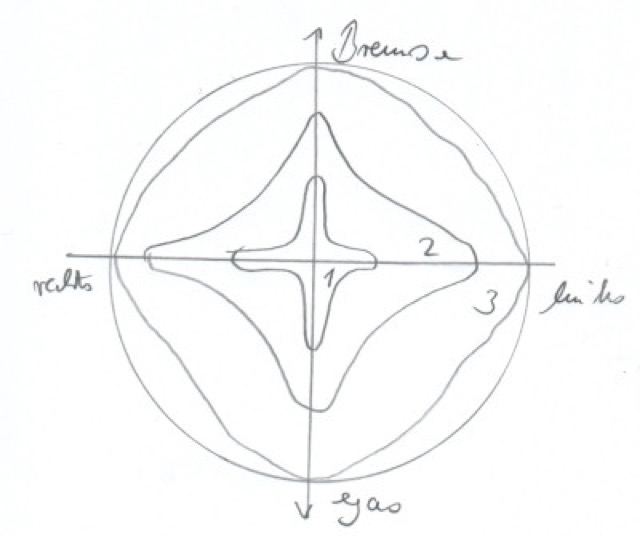
\includegraphics[width=0.5\textwidth]{images/kammsherkreis}
	\caption{Beschleunigungswerte einer Autofahrt dargestellt als Kammscher Kreis} \cite{FAIF.CH3-fahrkomfortanalyse.KammscherKreis}\label{Fig:Kammsher-Kreis}
\end{figure}

\subsubsection{Implementierung}

Bei der Umsetzung des Kammschen Kreisdiagrammes wurde erstmal die MPAndroidchart Libary verwendet.Da aber der Kammsche Kreis sich nicht mithilfe der Libary aktualisieren ließ wurde schnell die Lösung mittels canvas erstellt. 

Bei canvas ist es so, dass die onDraw Methode überschrieben werden muss um auf einer Fläche zeichnen zu können. Weiters habe ich mir eine Näherungsmethode erstellt womit ich die Punkte in 5er Winkel auf oder abrunde.


\lstinputlisting[caption=Runden-Methode, style=javastyle]{code/Runden.java}

\lstinputlisting[caption=Erstellung des Kammschen Kreises, style=javastyle]{code/ChartView.java}

